% Cover page — vLLM 推理引擎意象：中心 GPU 核心 + 辐射的 attention head
% 与 token 流，表现"并行注意力 + KV cache 流水线"概念。
% 纯矢量 TikZ，深绿线稿，完全可复现。
\begin{titlepage}
\thispagestyle{empty}
\begin{tikzpicture}[remember picture, overlay]
  \fill[structurecolor] (current page.north west) rectangle ([yshift=-0.85cm]current page.north east);
  \fill[structurecolor] (current page.south west) rectangle ([yshift=0.5cm]current page.south east);
\end{tikzpicture}
\centering
\vspace*{2.5cm}

{\fontsize{40}{50}\selectfont\rmfamily\bfseries vLLM 学习手册\par}
\vspace{0.6cm}
{\Large\sffamily\color{structurecolor} 源码级 LLM 推理工程教程\par}

\vspace{1.8cm}

% ── 推理引擎意象：GPU 核心 + attention head 矩阵 + token 流 ──
\begingroup
\definecolor{ink}{RGB}{30,99,65}
\definecolor{inklight}{RGB}{30,99,65}
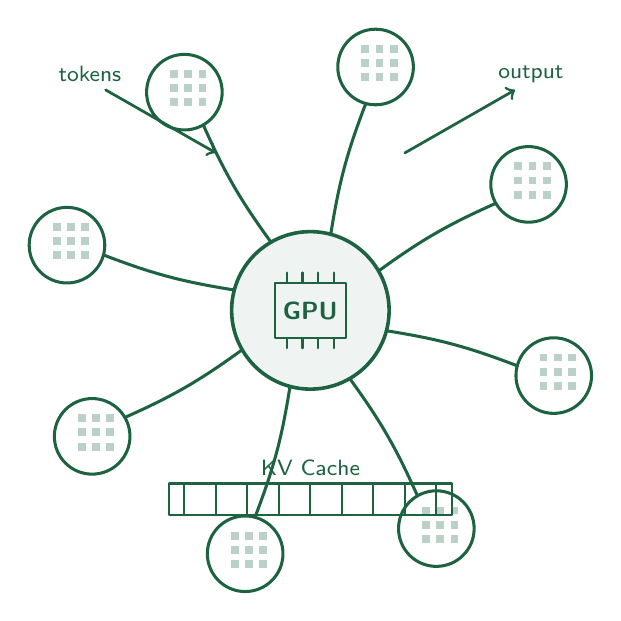
\begin{tikzpicture}[line join=round, line cap=round,
    arm/.style={ink, line width=1.1pt},
    ring/.style={ink, line width=1.1pt, fill=white},
    ic/.style={ink, line width=0.8pt}]
  \def\R{3.2}    % arm length
  \def\rh{1.0}   % hub radius

  % ── 外层 attention head 矩阵（小方块阵列，表现并行 attention）──
  \foreach \a in {30,75,120,165,210,255,300,345}{
    \begin{scope}[shift={(\a:\R)}]
      \draw[ring] (0,0) circle (0.48);
      % mini attention grid inside each head
      \foreach \dx in {-0.18,0,0.18}{
        \foreach \dy in {-0.18,0,0.18}{
          \fill[ink!30] (\dx,\dy) rectangle ++(0.10,0.10);
        }
      }
    \end{scope}
  }

  % arms connecting hub to heads
  \foreach \a in {30,75,120,165,210,255,300,345}{
    \draw[arm] (\a:\rh) to[bend left=6] (\a:\R-0.48);
  }

  % ── hub (GPU core) ──
  \fill[ink!7] (0,0) circle (\rh);
  \draw[ink, line width=1.3pt] (0,0) circle (\rh);
  % GPU chip motif: inner rectangle + pins
  \draw[ic] (-0.45,-0.35) rectangle (0.45,0.35);
  \foreach \p in {-0.30,-0.10,0.10,0.30}{
    \draw[ic] (\p,0.35) -- (\p,0.48);
    \draw[ic] (\p,-0.35) -- (\p,-0.48);
  }
  \node[ink] at (0,0) {\sffamily\bfseries\small GPU};

  % ── token flow arrows (left → hub → right) ──
  \draw[->,ink,line width=1.0pt] (-2.6,2.8) -- (-1.2,2.0);
  \node[ink] at (-2.8,3.0) {\sffamily\footnotesize tokens};
  \draw[->,ink,line width=1.0pt] (1.2,2.0) -- (2.6,2.8);
  \node[ink] at (2.8,3.0) {\sffamily\footnotesize output};

  % ── KV cache bar at bottom ──
  \draw[ink,line width=0.8pt] (-1.8,-2.6) rectangle (1.8,-2.2);
  \foreach \x in {-1.6,-1.2,-0.8,-0.4,0,0.4,0.8,1.2,1.6}{
    \draw[ic] (\x,-2.6) -- (\x,-2.2);
  }
  \node[ink] at (0,-2.0) {\sffamily\footnotesize KV Cache};

\end{tikzpicture}
\endgroup

\vfill
{\small\sffamily\color{structurecolor!80} 60 章 · 24K+ 行 · 源码对照锁定 commit\par}
\vspace{0.4cm}
{\small\sffamily\color{structurecolor!80} \number\year 年 \number\month 月\par}
\vspace{1.2cm}
\end{titlepage}
